\subsubsection{UC 11 - Stato Postazioni}

\begin{figure}[h]
  \centering
    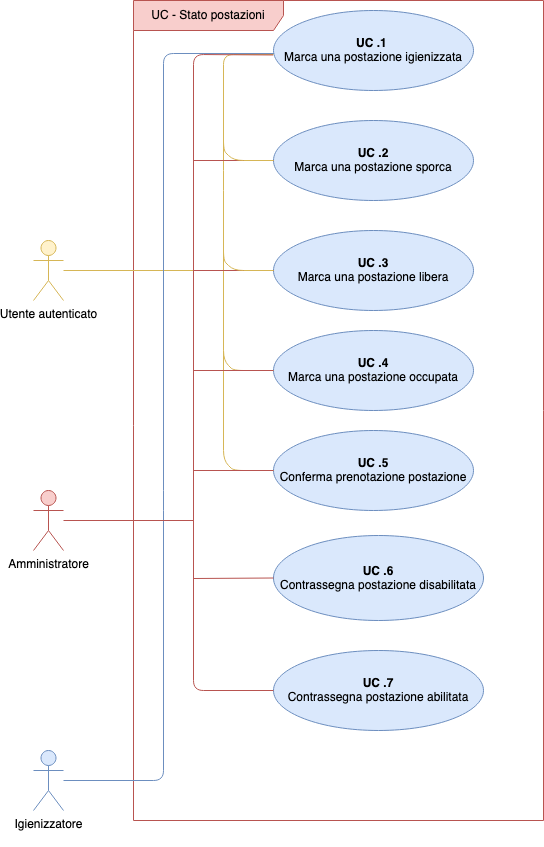
\includegraphics[scale=0.5]{src/CasiDUso/Immagini/UC11.png}
  \caption{UC11  - Stato prenotazioni}
\end{figure}

Il presente diagramma vuole riassumere la possibilità di prenotazione delle prenotazioni da parte di un utilizzatore dell’applicazione.

\begin{itemize}
\item \textbf{Attori primari:} utente autenticato, igienizzatore, amministratore;
\item \textbf{Descrizione:} l’utente può gestire le postazioni registrate nell’applicazione a cui ha accesso a livello di permessi, aggiungendo, rimuovendo, prenotando ed igienizzando ogni relativa postazione;
\item \textbf{Precondizione:} ogni utente è autenticato, e naviga nell’apposita sezione di gestione delle postazioni;
\item \textbf{Postcondizione:} l’utente ha gestito le proprie postazioni;
\item \textbf{Scenario principale:} 
	\begin{itemize}
		\item l’utente naviga nell’apposita sezione di gestione delle postazioni;
		\item l’utente visualizza e gestisce le postazioni a cui ha accesso.
	\end{itemize}
\end{itemize}

\subsubsection{UC11.1 - Marca postazione igienizzata}

\begin{itemize}
\item \textbf{Attori primari:} utente autenticato, igienizzatore, amministratore;
\item \textbf{Descrizione:} l’utente può marcare la postazione selezionata come igienizzata, quindi servibile ed occupabile da un successivo utente;
\item \textbf{Precondizione:} l’utente naviga nell’apposita sezione di gestione della postazione; 
\item \textbf{Postcondizione:} l’utente ha marcato con successo una postazione come igienizzata;
\item \textbf{Scenario principale:} 
	\begin{itemize}
		\item l’utente naviga nell’apposita sezione di gestione della postazione;		
		\item l’utente contrassegna la postazione come igienizzata;
		\item il sistema elabora correttamente la richiesta o, in alternativa, restituisce un errore, che può essere dovuto al seguente fattore:
		\begin{itemize}
			\item la postazione selezionata è stata marcata come disabilitata da un amministratore.
		\end{itemize}
	\end{itemize}
\end{itemize}

\subsubsection{UC11.2 - Marca postazione sporca}

\begin{itemize}
\item \textbf{Attori primari:} utente autenticato, amministratore;
\item \textbf{Descrizione:} l’utente può marcare la postazione selezionata come sporca, quindi non servibile ed occupabile da un successivo utente;
\item \textbf{Precondizione:} l’utente naviga nell’apposita sezione di gestione della postazione; 
\item \textbf{Postcondizione:} l’utente ha marcato con successo una postazione come sporca;
\item \textbf{Scenario principale:} 
	\begin{itemize}
		\item l’utente naviga nell’apposita sezione di gestione della postazione;		
		\item l’utente contrassegna la postazione come sporca;
		\item il sistema elabora correttamente la richiesta o, in alternativa, restituisce un errore, che può essere dovuto al seguente fattore:
		\begin{itemize}
			\item la postazione selezionata è stata marcata come disabilitata da un amministratore.
		\end{itemize}
	\end{itemize}
\end{itemize}

\subsubsection{UC11.3 - Marca postazione libera}

\begin{itemize}
\item \textbf{Attori primari:} utente autenticato, amministratore;
\item \textbf{Descrizione:} l’utente può marcare la postazione selezionata come libera, quindi servibile ed occupabile da un successivo utente;
\item \textbf{Precondizione:} l’utente naviga nell’apposita sezione di gestione della postazione;
\item \textbf{Postcondizione:} l’utente ha marcato con successo una postazione come libera;
\item \textbf{Scenario principale:} 
	\begin{itemize}
		\item l’utente naviga nell’apposita sezione di gestione della postazione;
		\item l’utente contrassegna la postazione come libera;
		\item il sistema elabora correttamente la richiesta o, in alternativa, restituisce un errore che può essere dovuto al seguente fattore:
		\begin{itemize}
			\item la postazione selezionata è stata marcata come disabilitata da un amministratore.
		\end{itemize}
	\end{itemize}
\end{itemize}

\subsubsection{UC11.4 - Marca postazione occupata}

\begin{itemize}
\item \textbf{Attori primari:} utente autenticato, amministratore;
\item \textbf{Descrizione:} l’utente può marcare la postazione selezionata come occupata, quindi non più occupabile da un altro utente;
\item \textbf{Precondizione:} l’utente naviga nell’apposita sezione di gestione della postazione;
\item \textbf{Postcondizione:} l’utente ha marcato con successo una postazione come occupata;
\item \textbf{Scenario principale:} 
	\begin{itemize}
		\item l’utente naviga nell’apposita sezione di gestione della postazione;
		\item l’utente contrassegna la postazione come occupata;
		\item il sistema elabora correttamente la richiesta o, in alternativa, restituisce un errore che può essere dovuto al seguente fattore:
		\begin{itemize}
			\item la postazione selezionata è stata marcata come disabilitata da un amministratore.
		\end{itemize}
	\end{itemize}
\end{itemize}

\subsubsection{UC11.5 - Conferma prenotazione della postazione}

\begin{itemize}
\item \textbf{Attori primari:} utente autenticato, amministratore;
\item \textbf{Descrizione:} l’utente è tenuto a confermare l’occupazione, e quindi la prenotazione, della postazione in uso;
\item \textbf{Precondizione:} l’utente conferma la sua prenotazione dall’apposita schermata pop-up; 
\item \textbf{Postcondizione:} l’utente ha confermato con successo la prenotazione della postazione;
\item \textbf{Scenario principale:} 
	\begin{itemize}
		\item l’utente contrassegna la postazione come occupata;
		\item il sistema elabora correttamente la richiesta.
	\end{itemize}
\end{itemize}

\subsubsection{UC11.6 - Contrassegna postazione disabilitata}

\begin{itemize}
\item \textbf{Attori primari:} amministratore;
\item \textbf{Descrizione:} l’amministratore può marcare la postazione selezionata come disabilitata, quindi non più servibile né occupabile da alcun utente;
\item \textbf{Precondizione:} l’amministratore naviga nell’apposita sezione di gestione della postazione;
\item \textbf{Postcondizione:} l’amministratore ha marcato con successo una postazione come disabilita;
\item \textbf{Scenario principale:} 
	\begin{itemize}
		\item l’amministratore naviga nell’apposita sezione di gestione della postazione;
		\item l’amministratore contrassegna la postazione come disabilitata;
		\item il sistema elabora correttamente la richiesta.
	\end{itemize}
\end{itemize}

\subsubsection{UC11.7 - Contrassegna postazione abilitata}

\begin{itemize}
\item \textbf{Attori primari:} amministratore;
\item \textbf{Descrizione:} l’amministratore può marcare la postazione precedentemente selezionata come “disabilitata”, nuovamente abilitata, quindi servibile ed occupabile da utenti;
\item \textbf{Precondizione:} l’amministratore naviga nell’apposita sezione di gestione della postazione; 
\item \textbf{Postcondizione:} l’amministratore ha marcato con successo una postazione, precedentemente disabilitata, come abilitata;
\item \textbf{Scenario principale:} 
	\begin{itemize}
		\item l’amministratore naviga nell’apposita sezione di gestione della postazione;
		\item l’amministratore contrassegna la postazione come abilitata;
		\item il sistema elabora correttamente la richiesta.
	\end{itemize}
\end{itemize}
